\documentclass{article}
\usepackage{nips07submit_e,times}
%\documentstyle[nips07submit_09,times]{article}
\usepackage{graphicx}

\usepackage{amssymb}

\title{Insert Title of Paper Here}


\author{
Matthew Faulkner\\
\\
\And
Jon Krause \\
\\
\And
Daniel Rosenberg \\
\\
}

% The \author macro works with any number of authors. There are two commands
% used to separate the names and addresses of multiple authors: \And and \AND.
%
% Using \And between authors leaves it to \LaTeX{} to determine where to break
% the lines. Using \AND forces a linebreak at that point. So, if \LaTeX{}
% puts 3 of 4 authors names on the first line, and the last on the second
% line, try using \AND instead of \And before the third author name.

\newcommand{\fix}{\marginpar{FIX}}
\newcommand{\new}{\marginpar{NEW}}

\begin{document}

%\makeanontitle
\maketitle

\begin{abstract}
Lorem ipsum dolor sit amet, consectetur adipiscing elit. Donec ac mattis augue. Vestibulum ante ipsum primis in faucibus orci luctus et ultrices posuere cubilia Curae; Morbi ut orci aliquam magna ultrices porttitor vel id enim. Praesent ut pharetra neque. Sed sit amet est at turpis blandit consequat. In sed libero sem. Aliquam erat volutpat. Curabitur ultrices nisi non augue congue volutpat. Cum sociis natoque penatibus et magnis dis parturient montes, nascetur ridiculus mus. Proin vitae felis sem. Pellentesque sit amet felis augue, et faucibus mauris. Duis a felis tellus, eu luctus neque. Suspendisse sed dapibus justo. In dolor mi, suscipit non malesuada eget, laoreet et nunc. Cras vestibulum, ipsum at tincidunt bibendum, arcu elit vehicula sapien, nec suscipit nisi mauris quis sem. Quisque sit amet eros nulla. Nunc viverra mollis scelerisque. Curabitur molestie hendrerit orci et pulvinar. Sed porta ultricies purus, ut molestie ligula dictum eu. Ut eget tellus at elit volutpat tempus. 
\end{abstract}

\section{Background}
Lorem ipsum dolor sit amet, consectetur adipiscing elit. Donec ac mattis augue. Vestibulum ante ipsum primis in faucibus orci luctus et ultrices posuere cubilia Curae; Morbi ut orci aliquam magna ultrices porttitor vel id enim. Praesent ut pharetra neque. Sed sit amet est at turpis blandit consequat. In sed libero sem. Aliquam erat volutpat. Curabitur ultrices nisi non augue congue volutpat. Cum sociis natoque penatibus et magnis dis parturient montes, nascetur ridiculus mus. Proin vitae felis sem. Pellentesque sit amet felis augue, et faucibus mauris. Duis a felis tellus, eu luctus neque. Suspendisse sed dapibus justo. In dolor mi, suscipit non malesuada eget, laoreet et nunc. Cras vestibulum, ipsum at tincidunt bibendum, arcu elit vehicula sapien, nec suscipit nisi mauris quis sem. Quisque sit amet eros nulla. Nunc viverra mollis scelerisque. Curabitur molestie hendrerit orci et pulvinar. Sed porta ultricies purus, ut molestie ligula dictum eu. Ut eget tellus at elit volutpat tempus. 

\section{Algorithms}
\subsection{Discretization Algorithms}
The simplest approach that one can take when tackling an infinite number of
arms is to merely pick out some finite number of arms and run a standard
finite-armed bandit algorithm on them.  This raises the following 
questions:
\begin{itemize}
\item How many arms should be chosen?
\item How should the arms be chosen?
\end{itemize}
The answer to the first question is algorithm- and problem-specific.  For
example, consider the case where the reward function $r(x) = x$ defined
on the interval $[0,1]$.  With no noise, the $\epsilon$-greedy strategy
will converge to the correct arm immediately after sampling each arm once,
and thus it is beneficial to choose a very large number of arms.  A
UCB1 or Exp3 strategy, though, will take significantly longer to
converge, so if convergence time is an issue, perhaps fewer arms should be
chosen at the expense of some accuracy.

Concerning how the arms themselves are chosen, two obvious strategies are
to either choose them randomly or to choose them in a grid (at regular
intervals in the 1D case).  Choosing the arms in a deterministic way
means that, for a fixed number of arms, we can construct a reward function
that makes the algorithm behave terribly.  Even given an arbitrary number
of arms, by choosing a reward function with a maximum near an endpoint of
an interval in $\mathbb{R}$, for example, we can ensure that the algorithm
would never do too well.  For these reasons, we opt to go with a random
choice of arms.

In any case, merely discretizing the domain into a finite number of arms
inctroduces a bias, as our effective hypothesis class (each of the arms)
probably no longer contains the optimal hypothesis.


\begin{figure}
 \centering
 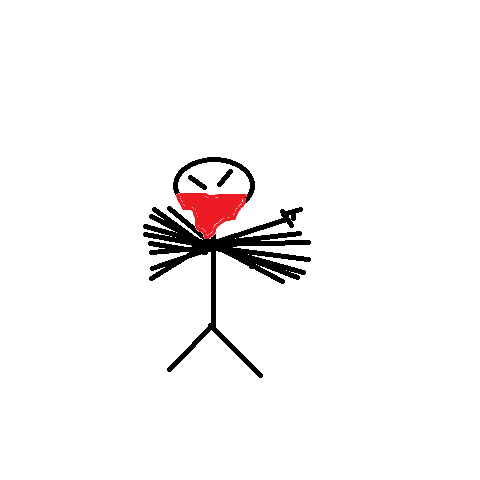
\includegraphics[width=240px]{./image.png}
 % image.png: 480x480 pixel, 72dpi, 16.93x16.93 cm, bb=0 0 480 480\
 \caption{Here we see a many armed bandit.}
 \label{manyarms}
\end{figure}


\subsection{Zooming Algorithm}
If you actually want to consider the infinite number of arms, you need to have certain information about the relationship between them. For instance, arms that are \emph{close} should produce similar results. The Zooming Algorithm is defined to work in any example where the arms form a metric space. In each phase, certain arms are chosen to be \emph{active}, and the algorithm chooses which arm to play from these active arms.

The Zooming Algorithm is composed of multiple phases, each of which is composed of $2^{i_{ph}}$ rounds, where $i_{ph}$ is the current phase number. In a given round, you \emph{activate} an arm if that arm is not covered by another arm. Each arm covers a radius defined by $r_t(v):=\sqrt{8*i_{ph}/(2+n_t(v)))}$ where $v$ is the active arm, and $n_t(v)$ is the number of times a given arm has been chosen at time $t$. Each time an arm is played, its radius shrinks, and at the beginning of each round, you \emph{activate} arms until you have a complete covering using a \emph{covering oracle}. This oracle can either return an uncovered arm, or state that there is no such arm. After the space is covered, you play the arm with the optimal index, defined as $I_t(v):=\mu_t(v)+2*r_t(v)$

A point of concern to us with this algorithm is that it does not seem to remember anything from previous phases when a new phase starts. The only piece of information it maintains is the phase number, which influeces the confidence radius and index, which changes the balance between exploration and exploitation. It seems like it may be better to start on a later phase, given knowledge of the specific problem. Aditionally, the \emph{covering oracle} becomes very complicated once you move into more advanced spaces.

\subsection{Hierarchical Optimistic Optimization}
Some very informative text

\section{Artificial Data Decription}
Real data? who needs it?
\\
\section{Possible Applications}
Apparently us.
\\
\section{Conclusion}
In conclusion, we did some stuff, and will do more.
\\
\section{Future Work}
hgjfjjh

\section*{References}


[1] Robert Kleinberg, Aleksandrs Slivkins, Eli Upfal, ``Multi-Armed Bandits in Metric Spaces''
\end{document}
